\chapter{Einleitung}
\label{chap:einleitung}
Dieses Kapitel gibt eine Übersicht über das Unternehmen \gls{arburg}. Nachfolgend wird die Aufgabenstellung aufgezeigt, deren Motivation erklärt sowie die Vorgehensweise geplant. 

\section{Unternehmensportrait}
\label{sec:unternehmen}
Das Familienunternehmen \gls{arburg} wurde 1923 von Arthur Hehl gegründet. Mittlerweile ist \gls{arburg} einer der weltweit führenden Hersteller von Spritzgießmaschinen zur Kunststoffverarbeitung. Das Stammwerk mit einer Fläche von 210.000 Quadratmetern befindet sich in Loßburg und ist Arbeitsplatz von rund 2.900 Mitarbeitern. Es handelt sich um den einzigen Produktionsstandort. Der Eigenfertigungsanteil der Produktion liegt bei circa 60\%. An knapp 100 Standorten weltweit sind insgesamt rund 600 weitere Mitarbeiter für Service, Vertrieb und Beratung angestellt. 2021 betrug der konsolidierte Umsatz 735 Millionen Euro. Im Portfolio von ARBURG befinden sich elektrische, hybride und hydraulische Spritzgießmaschinen (siehe \autoref{fig:maschinen} a), die \gls{allrounder} genannt werden. Außerdem zugehörige Peripherie und Robot-Systeme. Im Bereich der additiven Fertigung ergänzt seit 2013 der \gls{freeformer} (siehe \autoref{fig:maschinen} b) das Angebot der Firma.

\begin{figure}[!htb] 
	\centering
	\subfloat[\centering Spritzgießmaschine \gls{allrounder}]{{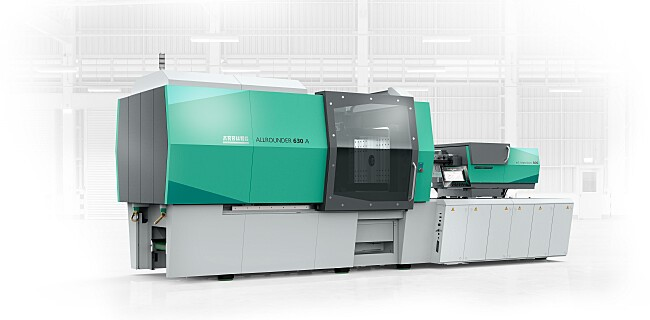
\includegraphics[width=7.8cm]{spritzgiessmaschine.jpg}}}%
	\qquad
	\subfloat[\centering \gls{freeformer}]{{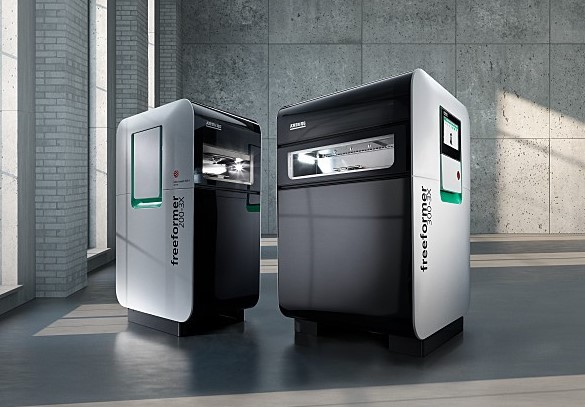
\includegraphics[width=5.5cm]{freeformer.jpg}}}%
	\caption{Produkte der Firma \gls{arburg} \cite{ARBURGGmbH+CoKG_Mediendatenbank}}%
	\label{fig:maschinen}%
\end{figure}
\FloatBarrier

Zur Bedienung der Maschinen ist die \gls{selogica} und seit 2016 auch die \gls{gestica} (siehe \autoref{fig:gestica_steuerung}) in Verwendung.

\begin{figure}[!htb] 
	\centering
		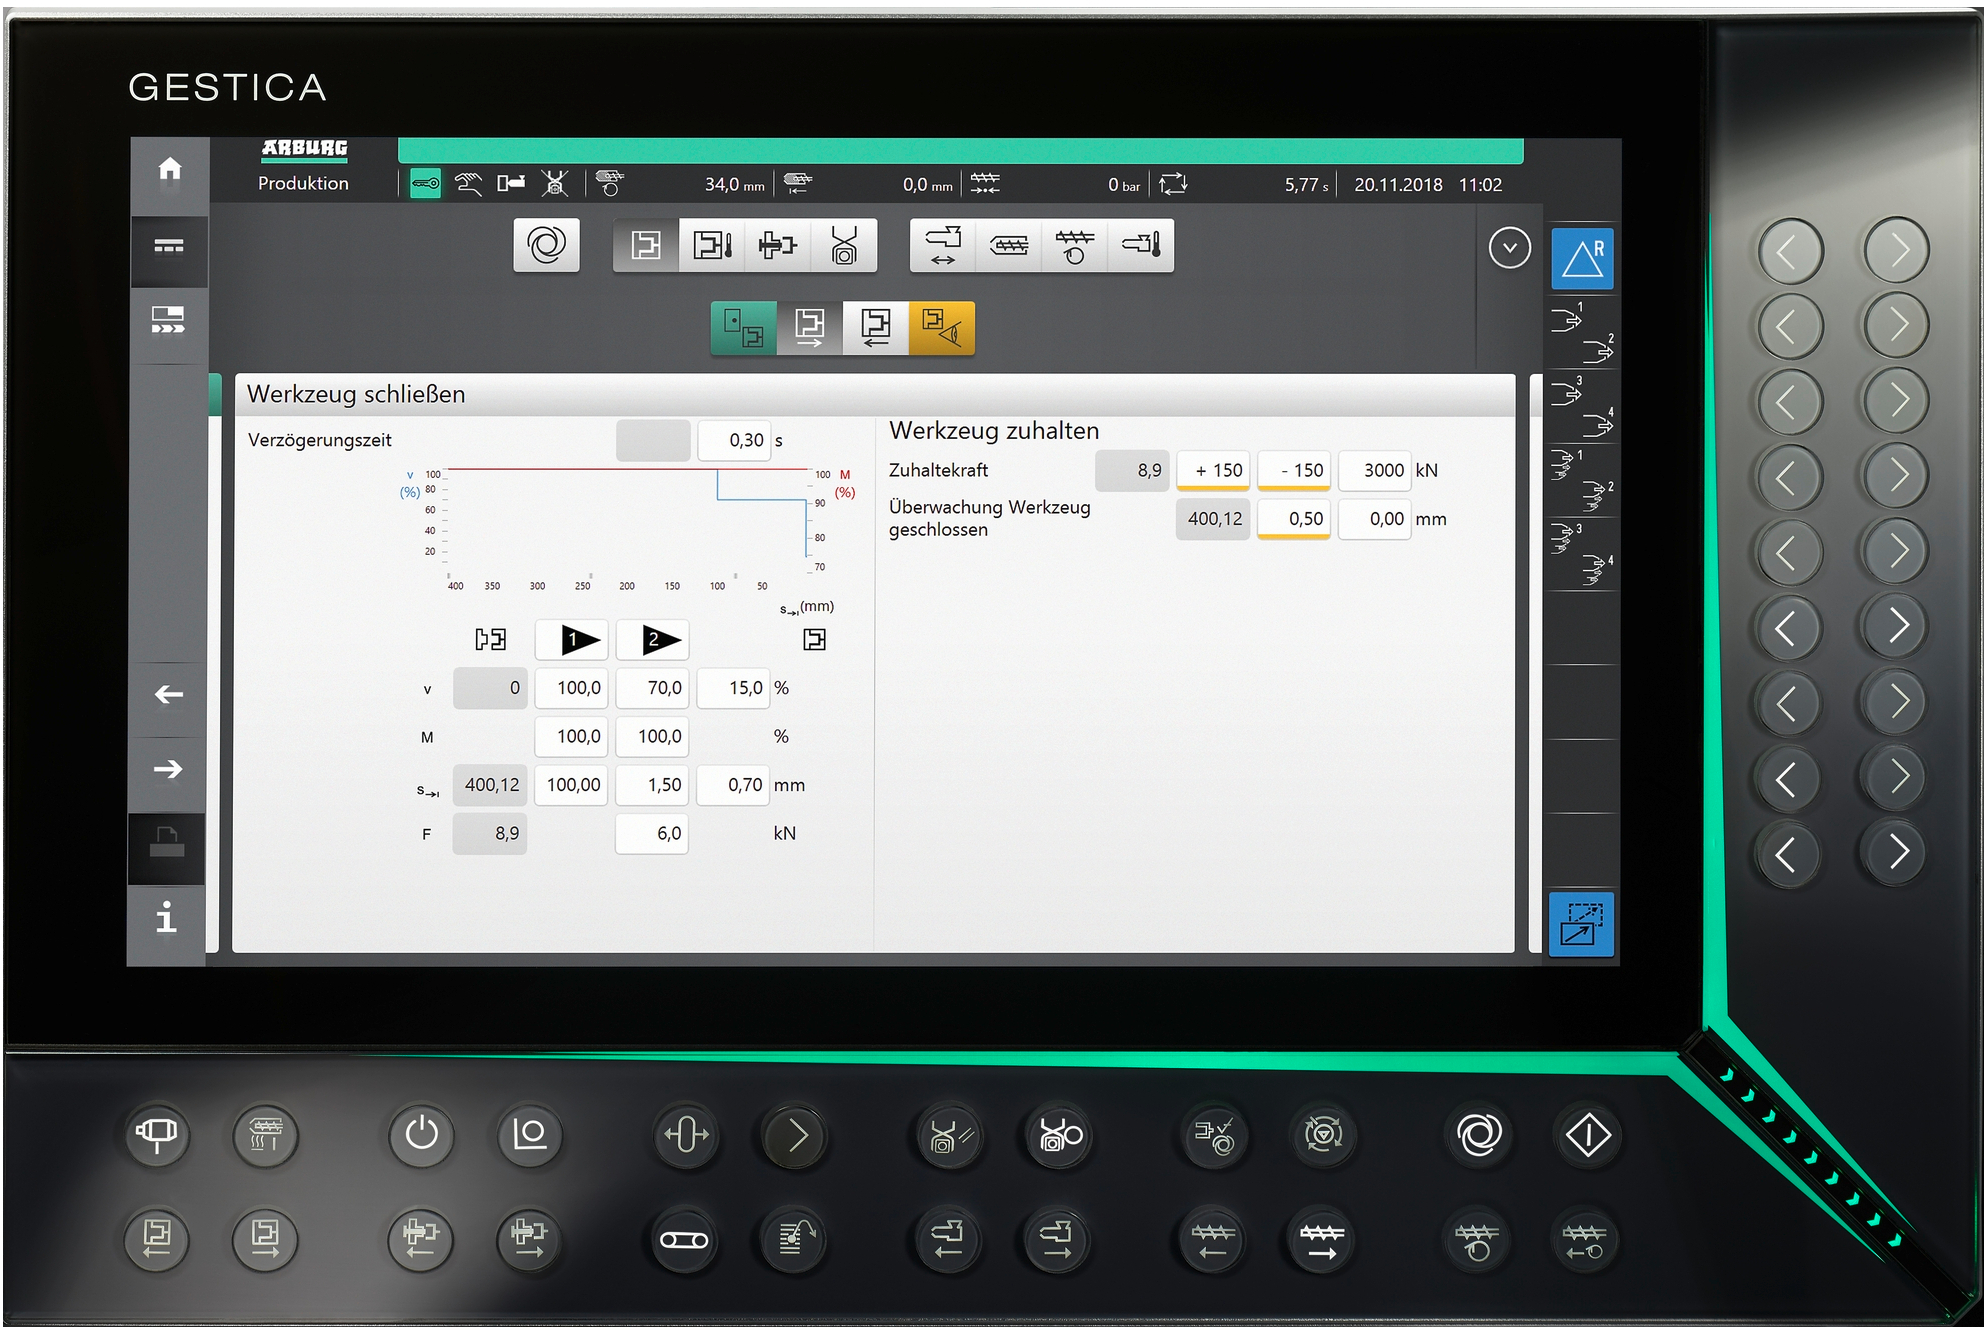
\includegraphics[width=8cm]{gestica.jpg}
	\caption{\gls{gestica} \cite{ARBURGGmbH+CoKG_Mediendatenbank}}
	\label{fig:gestica_steuerung}
\end{figure}
\FloatBarrier

\section{Motivation}
\label{motivation}
Seit Jahren nimmt die Spracherkennung- und Steuerung eine größere werdende Rolle ein. Bereits 2019 nutzen in Deutschland 51 Prozent der 18-24 Jährigen und etwa ein Drittel der 25-64 Jährigen einen Sprachassistenten per Smartphone \cite{Sprachassisten.2019}. Der Absatz von intelligenten Lautsprechern hat sich seit Anfang 2017 mehr als verzehnfacht \cite{SmarteLautsprecher.2021}. Auch im Unternehmen \gls{arburg} besteht der Wunsch, die Steuerung der Maschinen durch eine Sprachsteuerung zu verbessern. Aktuell ist dies nicht möglich. Dieser Wunsch ergibt sich aus dem Vorsatz, der Konkurrenz stets einen Schritt voraus zu sein und den aktuellen Stand der Technik voranzubringen. Grundgedanke ist die einfachere und schnellere Bedienung der Maschine für den Nutzer. Je nach Konzeption entfällt die Notwendigkeit für freie und saubere Hände, was die Wartung erleichtert. Die Implementierung eines solchen Features bietet dem Kunden einen Mehrwert und kann somit mehr Umsatz generieren. 

\section{Aufgabenstellung und Vorgehensweise}
\label{sec:aufgabevorgehen}
Aufgabe ist es, eine Sprachsteuerung für die \gls{arburg}-Maschinen zu konzeptionieren. Zunächst gibt eine Literaturrecherche Aufschluss darüber, wie verschiedene Spracherkennungen in der Theorie funktionieren und welche Chancen und Probleme dort auftreten können. Folgend werden unterschiedliche Anforderungen an ein Sprach-\gls{framework} definiert. Anhand dieser folgt eine Analyse verschiedener Software auf ihre Eignung. Schließlich findet die Auswahl der geeignetsten für die Nutzung im Hause \gls{arburg} statt. Außerdem werden Anforderungen für das Konzept der Sprachsteuerung definiert. Dies geschieht mithilfe des Befragens von Service-Technikern und Mitarbeitern des Schulungscenters. Diese haben zum einen direkten Kontakt mit dem Kunden und dessen Wünschen. Zum anderen kennen sie sich mit der Maschine aus und können daher die Sinnhaftigkeit verschiedener Ideen abschätzen. Dabei ist es nicht vorgesehen, jede Aktion auch durch einen Sprachbefehl ausführen zu können. Hier muss abgegrenzt werden, was sinnvoll und realistisch umzusetzen ist. Neben dem Ansteuern bereits vorhandener Funktionalitäten sollen, wenn notwendig, gegebenenfalls neue implementiert werden. Auf der anderen Seite dürfen gewisse Szenarien aufgrund von Sicherheitsaspekten nicht umgesetzt werden. Der Datenschutz stellt auch einen wichtigen Punkt zur Berücksichtigung dar. Anhand dieser Überlegungen und Anforderungen wird ein Konzept erstellt und eine Softwarearchitektur modelliert. Folgend findet eine Implementierung der Kernfunktionen statt. Tests in verschiedenen Lärmumgebungen sollen Aufschluss über die Performance geben.

\section{Ziel der Arbeit}
\label{sec:ziel}
Ziel der Arbeit ist die Auswahl einer Software sowie die Erstellung eines Konzeptes zur Nutzung einer Spracherkennung in der \gls{gestica}. Das Konzept muss dabei realisierbar, sinnvoll und zukunftsfähig sein, da die Entwicklung im Bereich der Spracherkennung noch nicht zu Ende ist. Das Endprodukt hat daher den Aspekten Austauschbarkeit, Veränderbarkeit und Erweiterbarkeit zu genügen. Kernkomponenten des Konzeptes werden dabei prototypisch implementiert. Anhand dieser Implementierung wird ein Fazit über die Sinnhaftigkeit der Sprachsteuerung für \gls{arburg} gezogen. In diesem sollen folgende Fragen geklärt sein.
\begin{itemize}
	\item Ist eine passende Software verfügbar?
	\item Ist die ausgewählte Software ausreichend oder muss gegebenenfalls eine andere verwendet und daher Anforderungen an diese verändert werden?
	\item Erlaubt die \gls{gestica}-Infrastruktur ein problemloses Einbinden der Sprachsteuerung?
	\item Ist eine Sprachsteuerung in lauten Umgebungen überhaupt nutzbar?
	\item Gibt es genug Use Cases um eine vollständige Implementierung des Konzeptes zu rechtfertigen?
\end{itemize}